\chapter{无监督机器学习方法的尝试}
\section{引言}

聚类分析是无监督学习的一种,旨在发现数据间是否有潜在的相似性\cite{Liu2018}。
因此,我们做了额外的探究——在不给定脉搏波对应的子痫前期的数据标签的基础上,探究能否有效的将数据分成两类,并考察验证分类的效果。

本文进行了以下探究:
1.	分别使用基于ppg 特征的$ppg_feature$ 数据与基于ppg波形数据的$ppg_points $数据,使用sklearn的kmeans 方法进行了聚类分析,其中超参数$n_clusters$被设置为2。
此时,此时若我们将聚类结果作为其学习的分类结果,与数据对应的数据标签进行对照,也可以得到混淆矩阵分别如下

之所以每种分析会得到两个混淆矩阵,是因为聚类分析的簇是不带标签的。两个混淆矩阵是给予簇不同的标签(健康或子痫)。为分析方便,我们选取准确率高的一种聚类结果,即上表中的2、3。并在此基础上进行后续分析。

2.	从表格中可以看到两种数据的聚类分析的准确率分别达到了61.6\%与51.5\%。
基于特征的聚类效果优于直接使用脉搏波波形数据的。
其次,乍一看,数据分类效果并不太好。特别是后者的准确率堪堪超过50\%(典型的随机分类的效果)
但是,我们需要注意到聚类分析的本质是根据数据特征的相似度,也即数据波形的相似度。
因此,让我们来考察下划分出来的波形究竟如何。
于是,我们把图画出来。

此外,我们还需要注意到另外一个变量因素,在PE的影响下,所有患病孕妇的数据波形是会受到影响的,而与正常波形形态有异。因此,所有PE患者都受到了一定程序的医学干预(包括不限于降血压等治疗),目的是使PE患者能够恢复正常水平。因此,会出现假阴性远高于假阳性的现象。可以总结为,在PE确实能改变孕妇脉搏波波形的前提下,聚类分析中出现的假阴性高于假阳性证明是医学干预的必然结果。分析数据与理论分析保持一致。
3.	到具体波形

\begin{figure}[htbp]
    \centering
    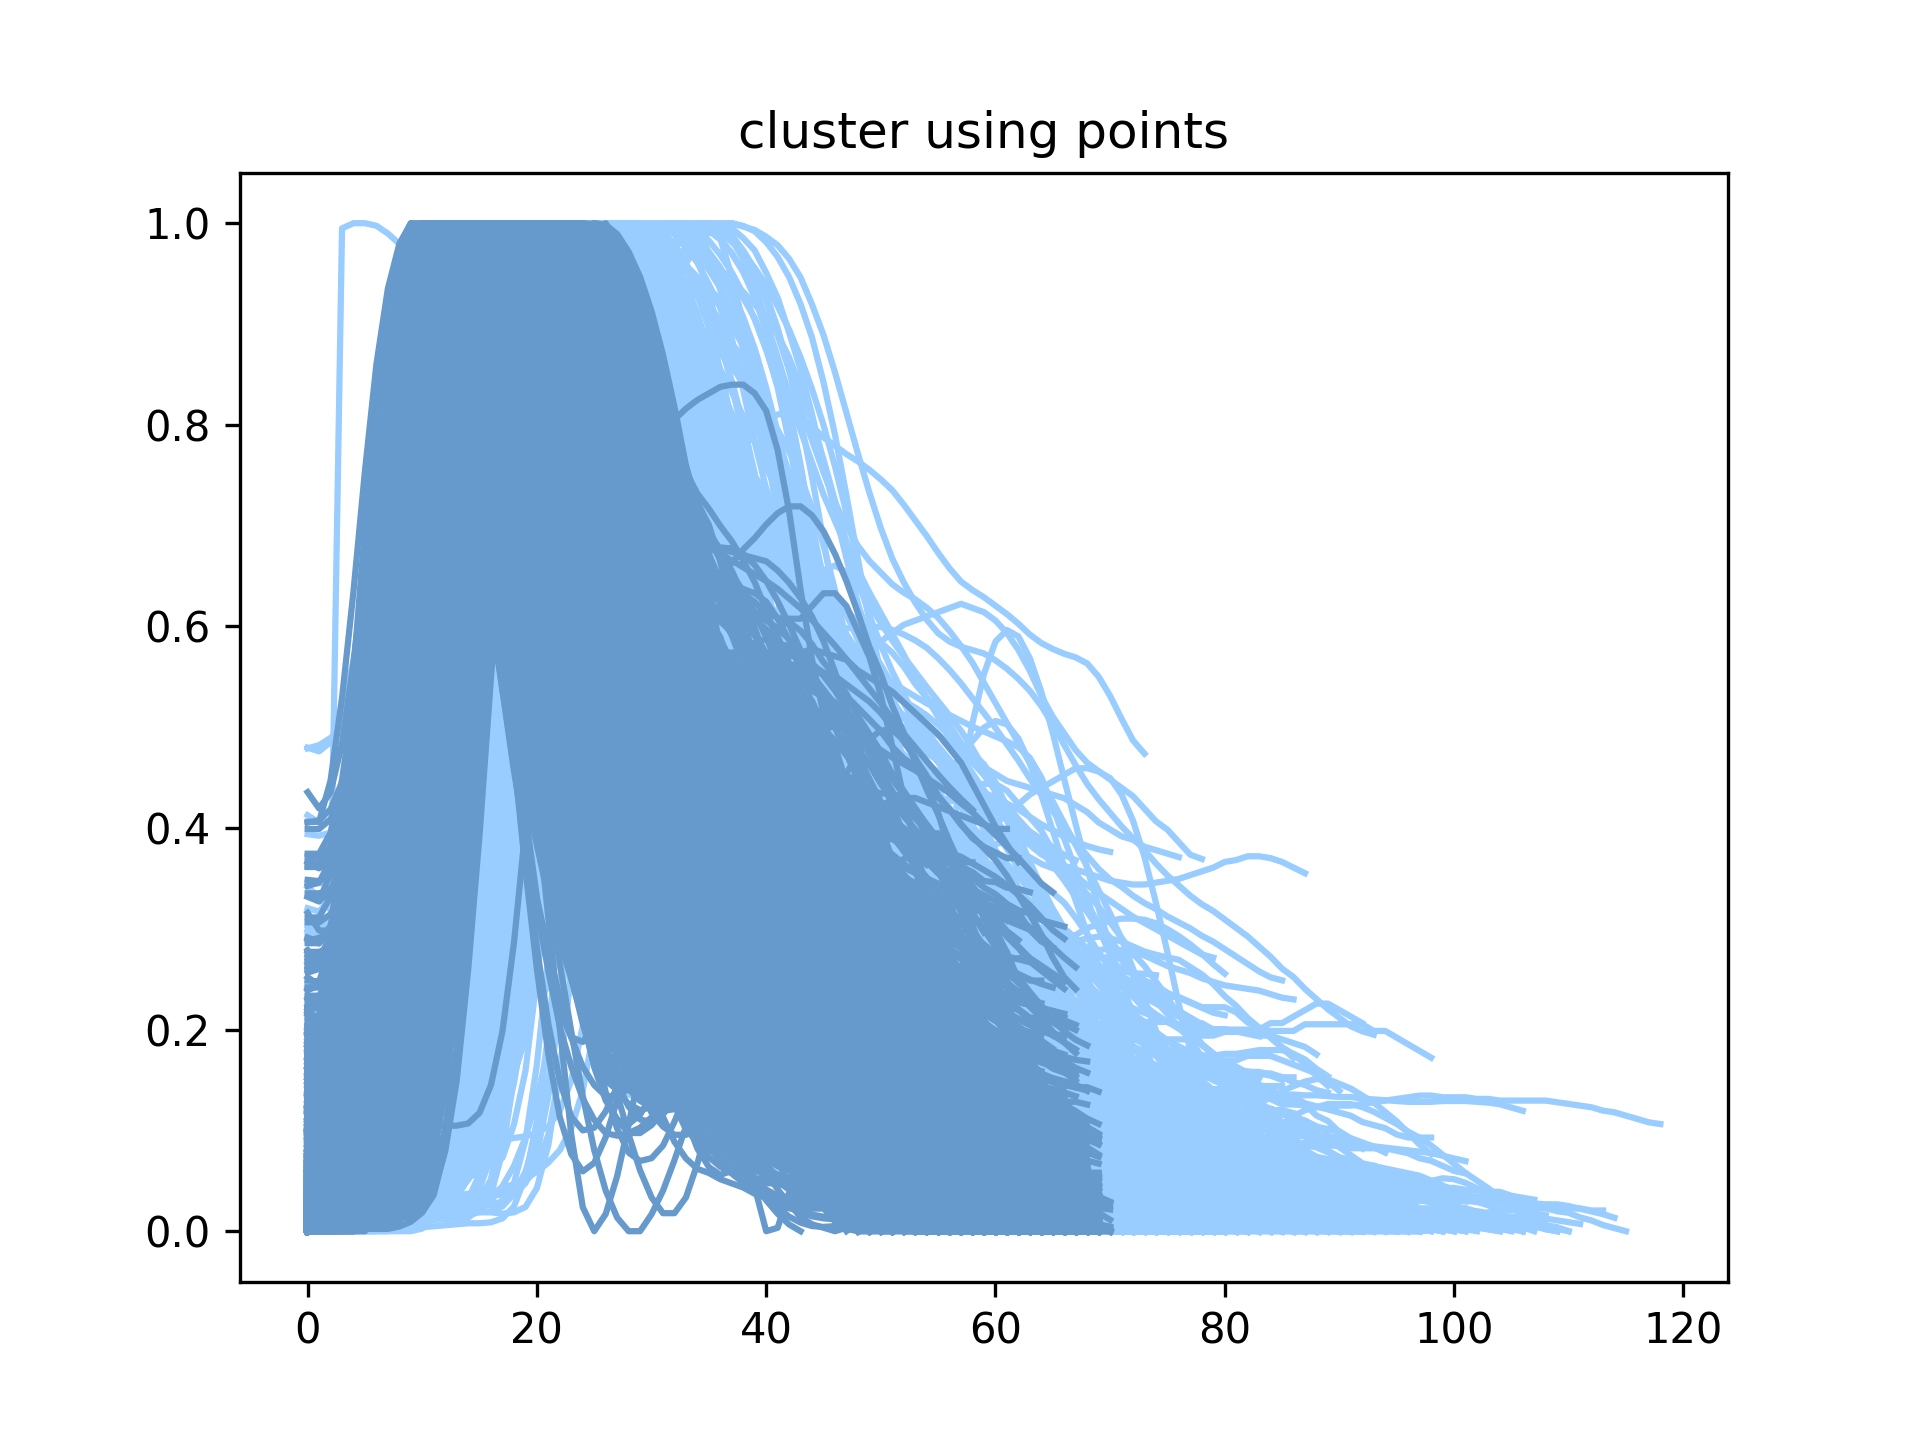
\includegraphics[width=.6\linewidth]{unsupervised/cluster using points_2d}
    \caption[]{\label{fig:cluster2d}111}
\end{figure}
\begin{figure}[htbp]
    \centering
    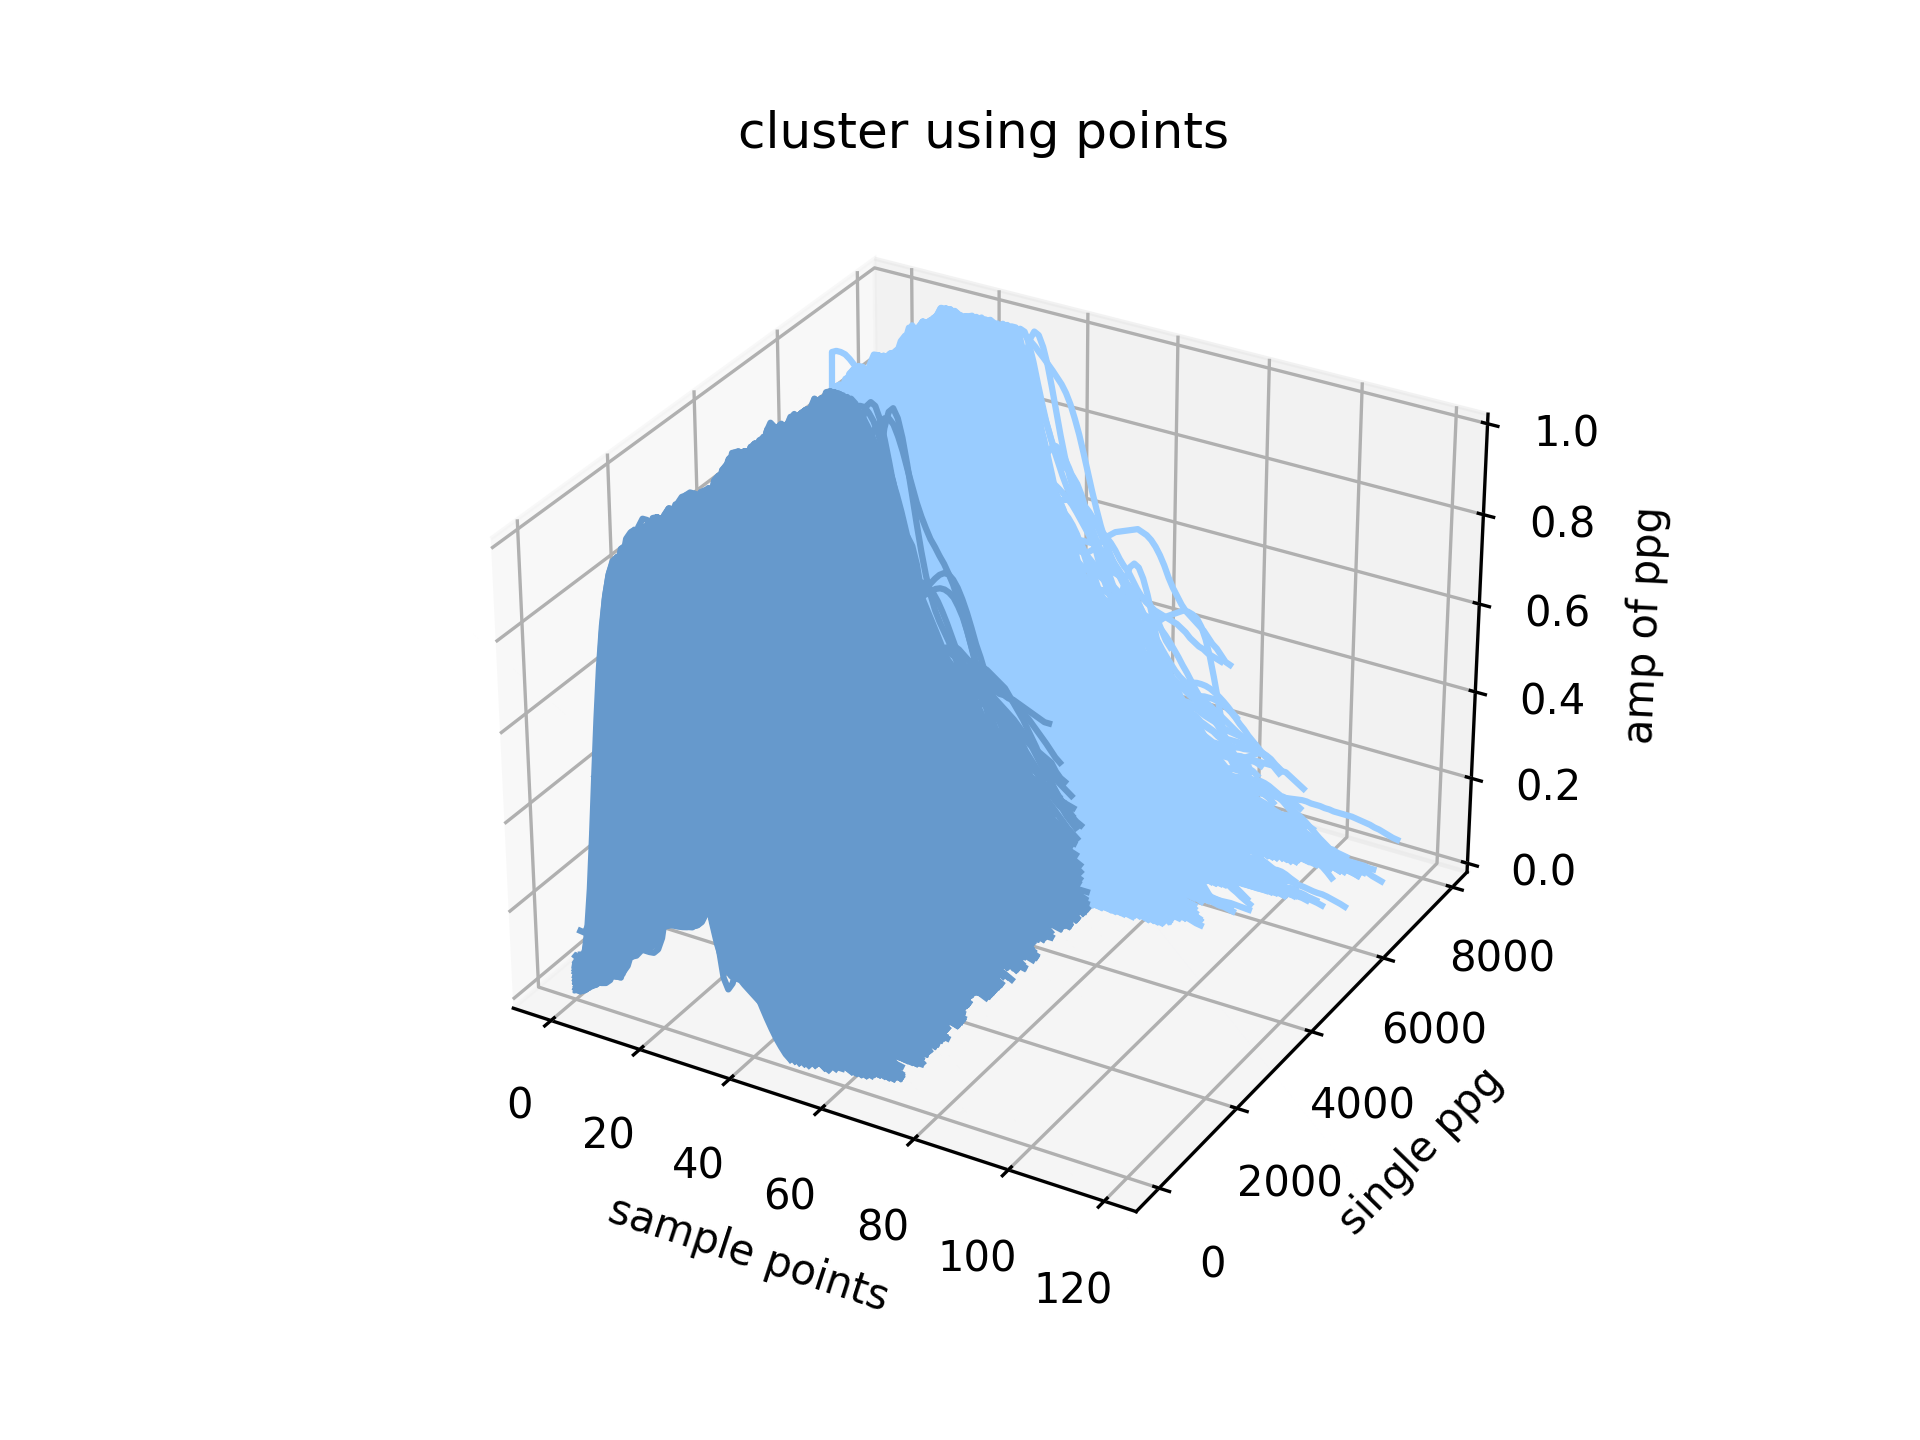
\includegraphics[width=.7\linewidth]{unsupervised/cluster using points_3d}
    \caption[]{\label{fig:cluster3d}222}
\end{figure}
\section{对k的调整与探索}
\section{集成学习的应用}
\section{深度学习模型的应用}
\section{小结}
